\section{Optimal Mass Transport}

In this section,we extend the optimal mass transport theory algorithm framework \cite{gu2013variational} \cite{su2017volume} to address the data injection division problem. 

\vspace*{20pt}

The original method depends on the rigorous geometry structure,yet in the real application,the implementation is hard and not stable because of the numerical calculation errors. \\

I re-implement this framework using Monte Carlo method, which can be extend to $N$ dimension. In addition, the implement is simple and we get the appropriate accurate effect as adding more sampling points.
\\

Let's consider two situations as example.
\begin{itemize}
\item Given an initial division,try to redivide the regular mesh to even division using the minimum cost. For example, the number of unit core ratio of 10 pieces is [0.4 0.4 0.4 0.4 0.4 0.4 0.4 0.4 0.4 0.4]
\item Give an initial division,try to redivide the regular mesh to a target measure division using the minimum cost.For example,the number of unit core ratio of 10 pieces is [0.4 0.3 0.3 0.4 0.2 0.2 0.3 0.4 0.7 0.9]
\end{itemize}



\subsection{Situation 1}

The initial division as follows Fig.\ref{voronoiinit}:

\begin{figure}[h]
\centering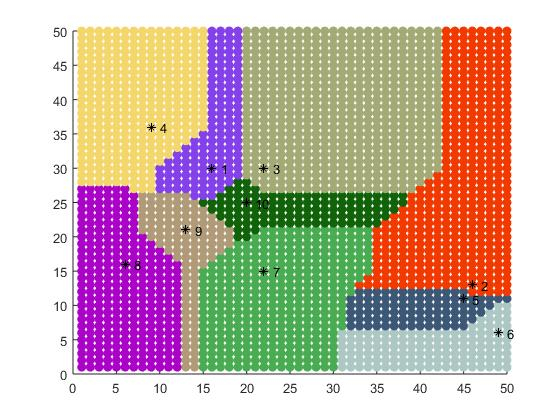
\includegraphics[width=0.8\linewidth]{figure/voronoiinit}
\caption{50*50 regular mesh with 10 data injection community division}
\label{voronoiinit}
\end{figure}

\vspace*{30pt}
The optimal mass transport even division as follows Fig.\ref{omtcell}:

\begin{figure}[h]
\centering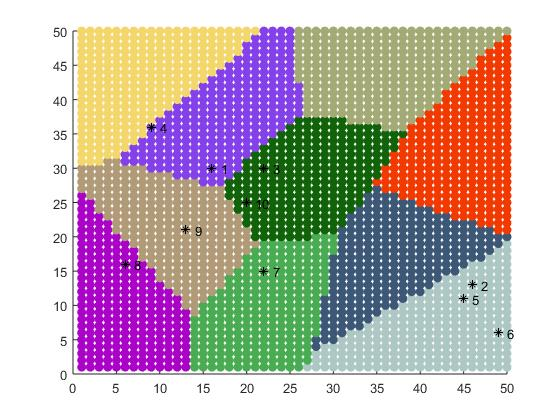
\includegraphics[width=0.8\linewidth]{figure/omtcell}
\caption{50*50 regular mesh with 10 data injection community division}
\label{omtcell}
\end{figure}
\vspace*{30pt}

After re-choose the data injection position as follows Fig.\ref{omtcell2}:
\begin{figure}[h]
\centering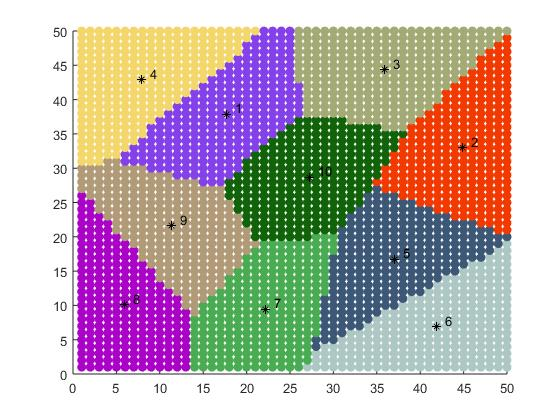
\includegraphics[width=0.8\linewidth]{figure/omtcell2}
\caption{50*50 regular mesh with 10 data injection community division}
\label{omtcell2}
\end{figure}

\vspace*{30pt}

The speedup ratio as follows:\\

The initial speedup figure. Fig.\ref{voronoicurve}
\\

\begin{figure}[h]
\centering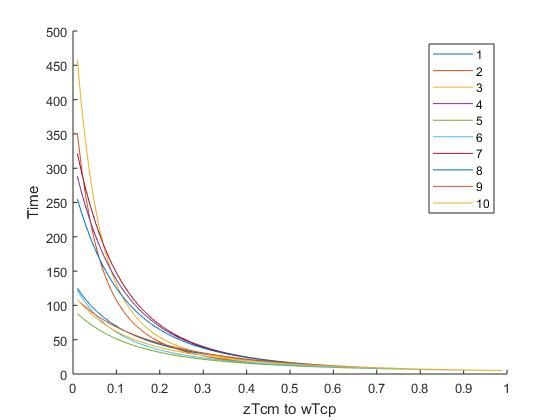
\includegraphics[width=0.8\linewidth]{figure/voronoicurve}
\caption{Speedup vs $\sigma$ in different community division}
\label{voronoicurve}
\end{figure}


Re-balance optimize speedup figure Fig.\ref{voronoicurve2}
\\

\begin{figure}[h]
\centering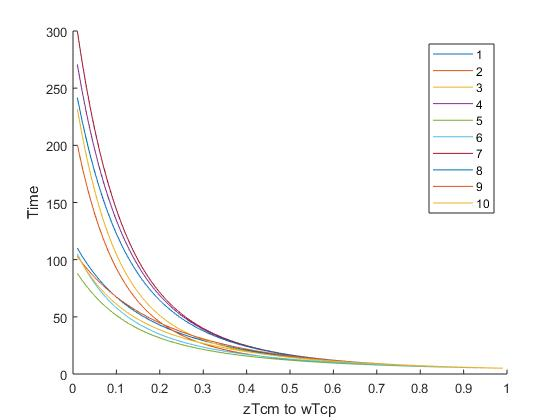
\includegraphics[width=0.8\linewidth]{figure/voronoicurve2}
\caption{Speedup vs $\sigma$ in different community division}
\label{voronoicurve2}
\end{figure}


The optimal mass transport speedup figure Fig.\ref{voronoicurve3}
\\

\begin{figure}[h]
\centering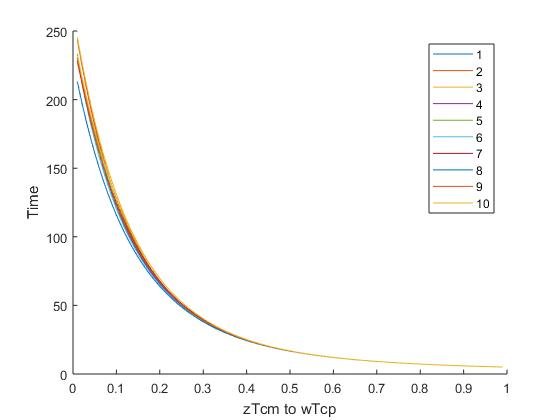
\includegraphics[width=0.8\linewidth]{figure/voronoicurve3}
\caption{Speedup vs $\sigma$ in different community division}
\label{voronoicurve3}
\end{figure}

\subsection{Situation 2}

\begin{figure}[h]
\centering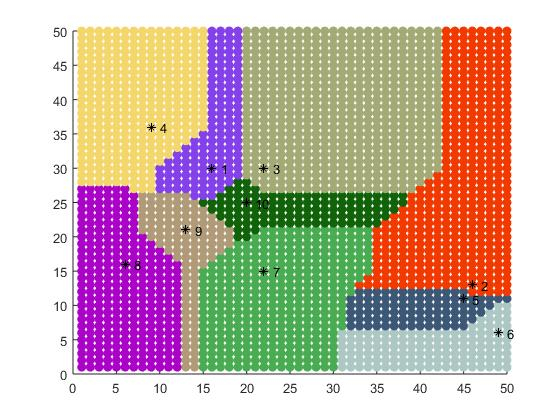
\includegraphics[width=0.8\linewidth]{figure/voronoiinit}
\caption{50*50 regular mesh with 10 data injection community division}
\label{voronoiinit}
\end{figure}

The optimal mass transport even division as follows:
\\

\begin{figure}[h]
\centering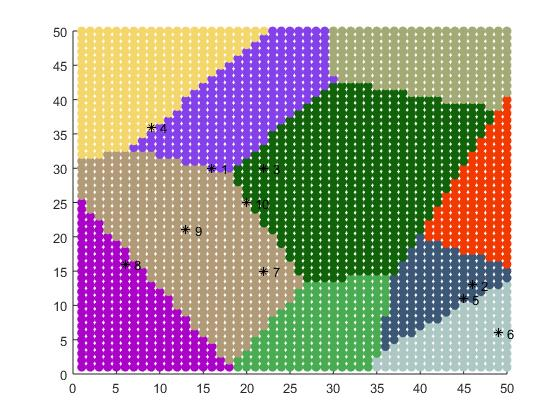
\includegraphics[width=0.8\linewidth]{figure/2omtcell}
\caption{50*50 regular mesh with 10 data injection community division}
\label{2omtcell}
\end{figure}

After re-choose the data injection position as follows:
\\
\begin{figure}[h]
\centering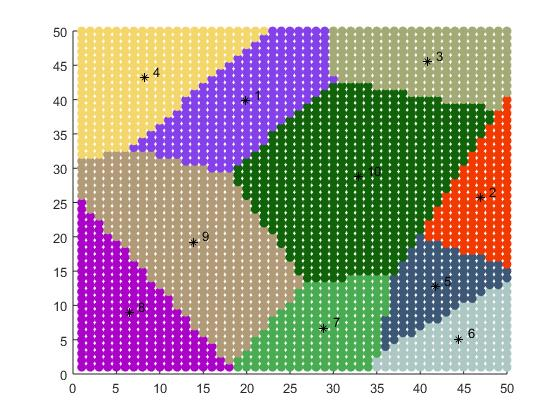
\includegraphics[width=0.8\linewidth]{figure/2omtcell2}
\caption{50*50 regular mesh with 10 data injection community division}
\label{2omtcell2}
\end{figure}

The speedup ratio as follows:
\\
The initial speedup figure. Fig.\ref{2voronoicurve}

\begin{figure}[h]
\centering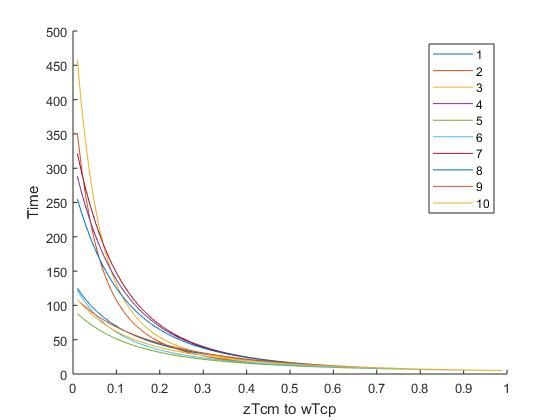
\includegraphics[width=0.8\linewidth]{figure/2voronoicurve}
\caption{Speedup vs $\sigma$ in different community division}
\label{2voronoicurve}
\end{figure}

Re-balance Voronoi optimization speedup figure Fig.\ref{2voronoicurve2}
\\
\begin{figure}[h]
\centering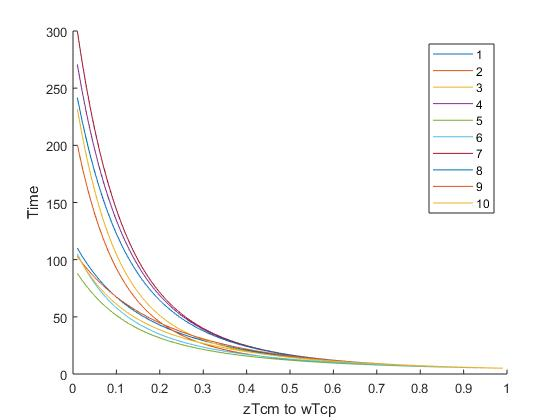
\includegraphics[width=0.8\linewidth]{figure/2voronoicurve2}
\caption{Speedup vs $\sigma$ in different community division}
\label{2voronoicurve2}
\end{figure}

The optimal mass transport speedup figure Fig.\ref{2voronoicurve3}
\\
\begin{figure}[h]
\centering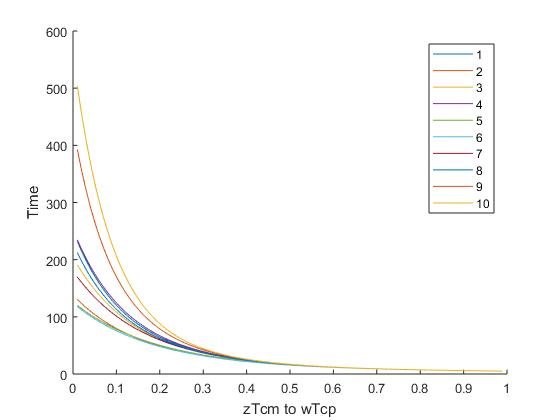
\includegraphics[width=0.8\linewidth]{figure/2voronoicurve3}
\caption{Speedup vs $\sigma$ in different community division}
\label{2voronoicurve3}
\end{figure}
